\documentclass[a4paper]{article}

\renewcommand{\labelenumii}{\theenumii}
\renewcommand{\theenumii}{\theenumi.\arabic{enumii}.}

\usepackage{fullpage} % Package to use full page
\usepackage{parskip} % Package to tweak paragraph skipping
\usepackage{tikz} % Package for drawing
\usepackage{amsmath}
\usepackage{amssymb,amsthm}
\usepackage{mathtools}
\usepackage{hyperref}
\usepackage{enumitem}
\usepackage{mathtools}
\usepackage{empheq}
\usepackage{amsfonts}
\usepackage{gensymb}
\usepackage{float}
\usepackage{subcaption}
\usepackage{placeins}

\newcommand*\widefbox[1]{\fbox{\hspace{2em}#1\hspace{2em}}}
%======================================== Title===========================================
\newcommand{\horrule}[1]{\rule{\linewidth}{#1}} 	% Horizontal rule
\title{
		\vspace{-0.6in} 	
		\usefont{OT1}{bch}{b}{n}
		\normalfont \normalsize \textsc{University of California Santa Cruz} \\ [10pt]
		\horrule{0.5pt} \\[0.4cm]
		\huge CMPE264 Proyect 1: High Dynamic Range (HDR) System \\
		\horrule{2pt} \\[0.5cm]
}
\author{
		\normalfont 								
        Aaron Hunter\\  Carlos Espinosa\\[-3pt]		\normalsize
        November 14, 2018
}
\date{}
%====================================Begin document=======================================
\begin{document}
\maketitle
%-----------------------------------------------------------------------------------------S1
\section{Camera Radiometric Calibration}
First we need to reverse-engineer the function $f(\cdot)$ and invert it, obtaining an approximation of the true (linear) brightness $B=f-1(B')$.
%-----------------------------------------------------------------------------------------
\section{Picture Stack Acquisition}
Now weed to take a stack of 3 images of a high-dynamic (high contrast) scene, so we proceed to take a stack of multiple pictures at different exposure time $T$ with fixed ISO gain $G$ and based on their corresponding histograms we can decide which 3 pictures to extract from this stack.

\begin{figure}[H]
\centering
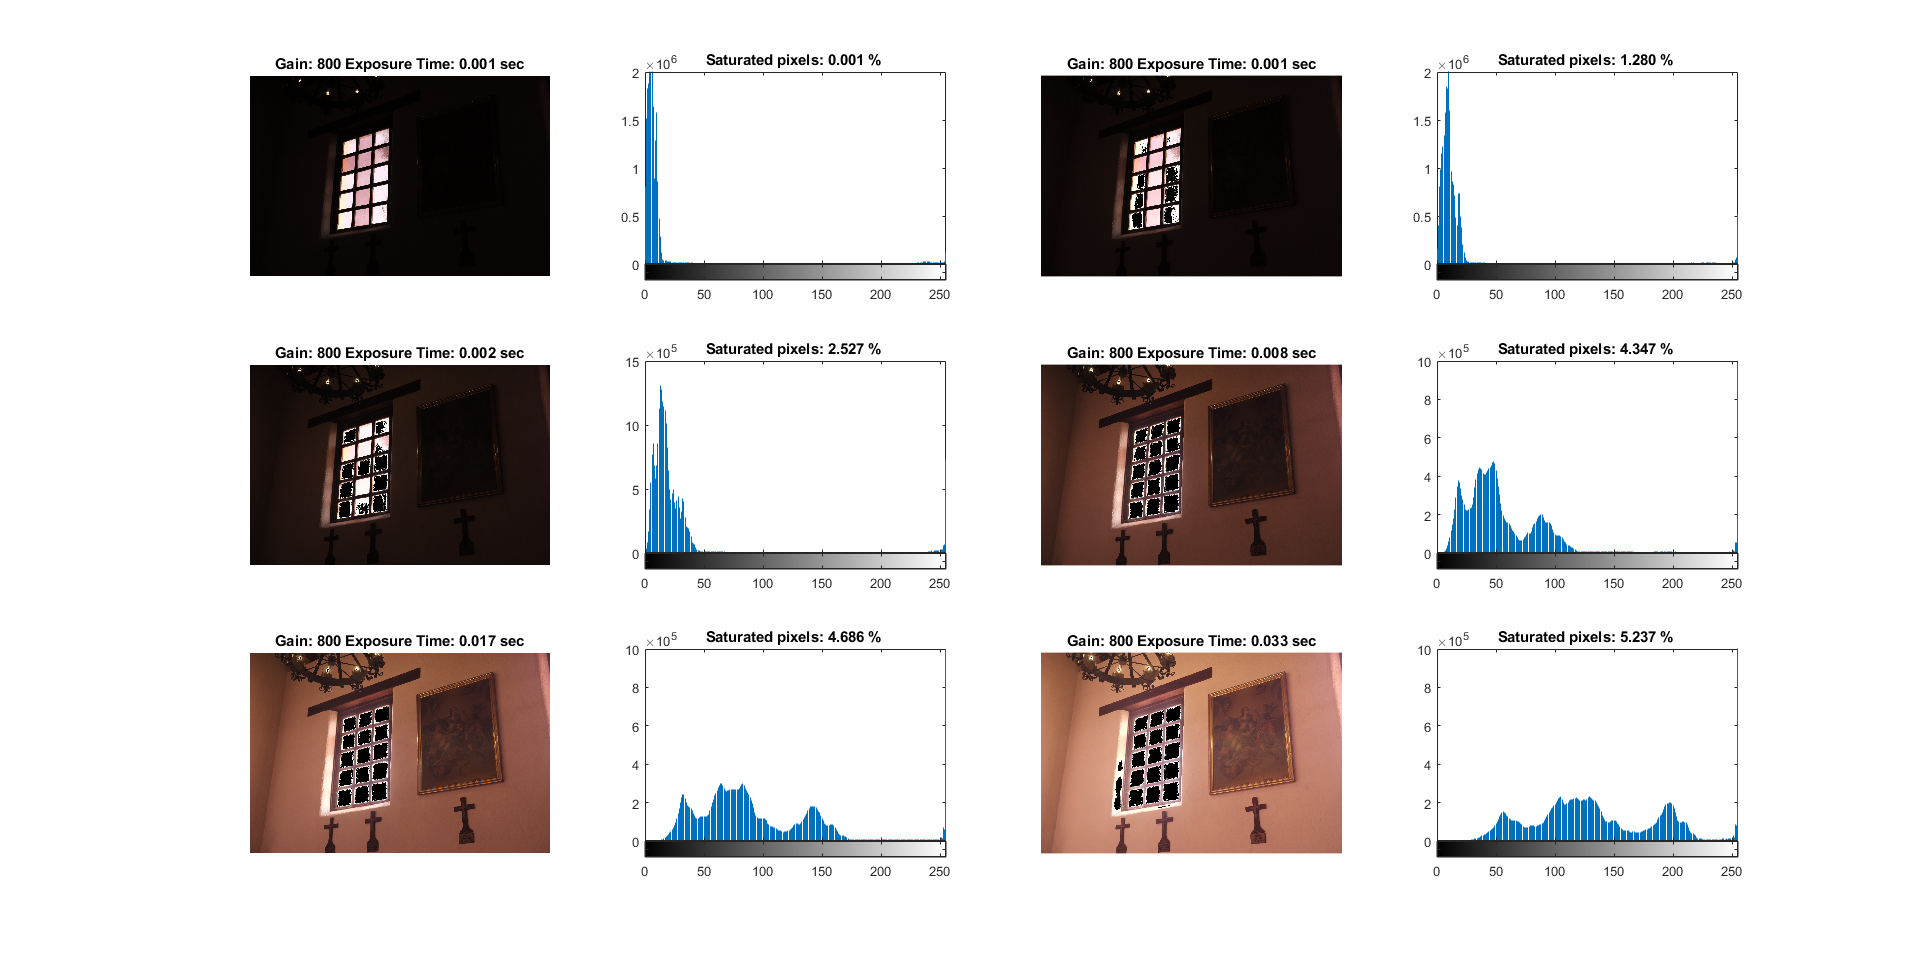
\includegraphics[trim=7cm 1cm 1cm 0cm clip, scale=.4]{Chapel_Histogram_set.png}
\caption{Picture Stack with ISO gain fixed at $G = 800$}
\label{fig:PicStack}
\end{figure}
\FloatBarrier
%-----------------------------------------------------------------------------------------S2
\section{Composite Image Creation}
We proceed to create a composite HDR image from our stack of three linearized pictures. We will compose the images using two different algorithms.

\subsection{Composition Algorithm 1}

\subsection{Composition Algorithm 2}
%-----------------------------------------------------------------------------------------S3
\section{Composite Image Reproduction}
Now we need to revert the linearization by applying a non-linear function that will amplify the small values and reduce the large values
%-----------------------------------------------------------------------------------------S4
\section{Script Execution}

\subsection{Requirements}
%-----------------------------------------------------------------------------------------S5
\section{Conclusions}


%%% End document
\end{document}